\subsection{Resultado - Exercício 2}

Os passos são:
\begin{itemize}[leftmargin=3.5em, itemsep=-.5mm, topsep=0.5mm]
    \item Derivar $f^{(k)}(t)$ de forma genérica
    \item Descobrir quanto vale $f^{(k)}(0)$ de forma genérica.
    \item Expandir para a Série de taylor para forma genérica
    \item Gerar tabela para comparação
    \item Apresentar o código Python
 \end{itemize}

\subsubsection{Derivar $f^{(k)}(t)$ de forma genérica}

\begin{figure}[H]
    \centering
    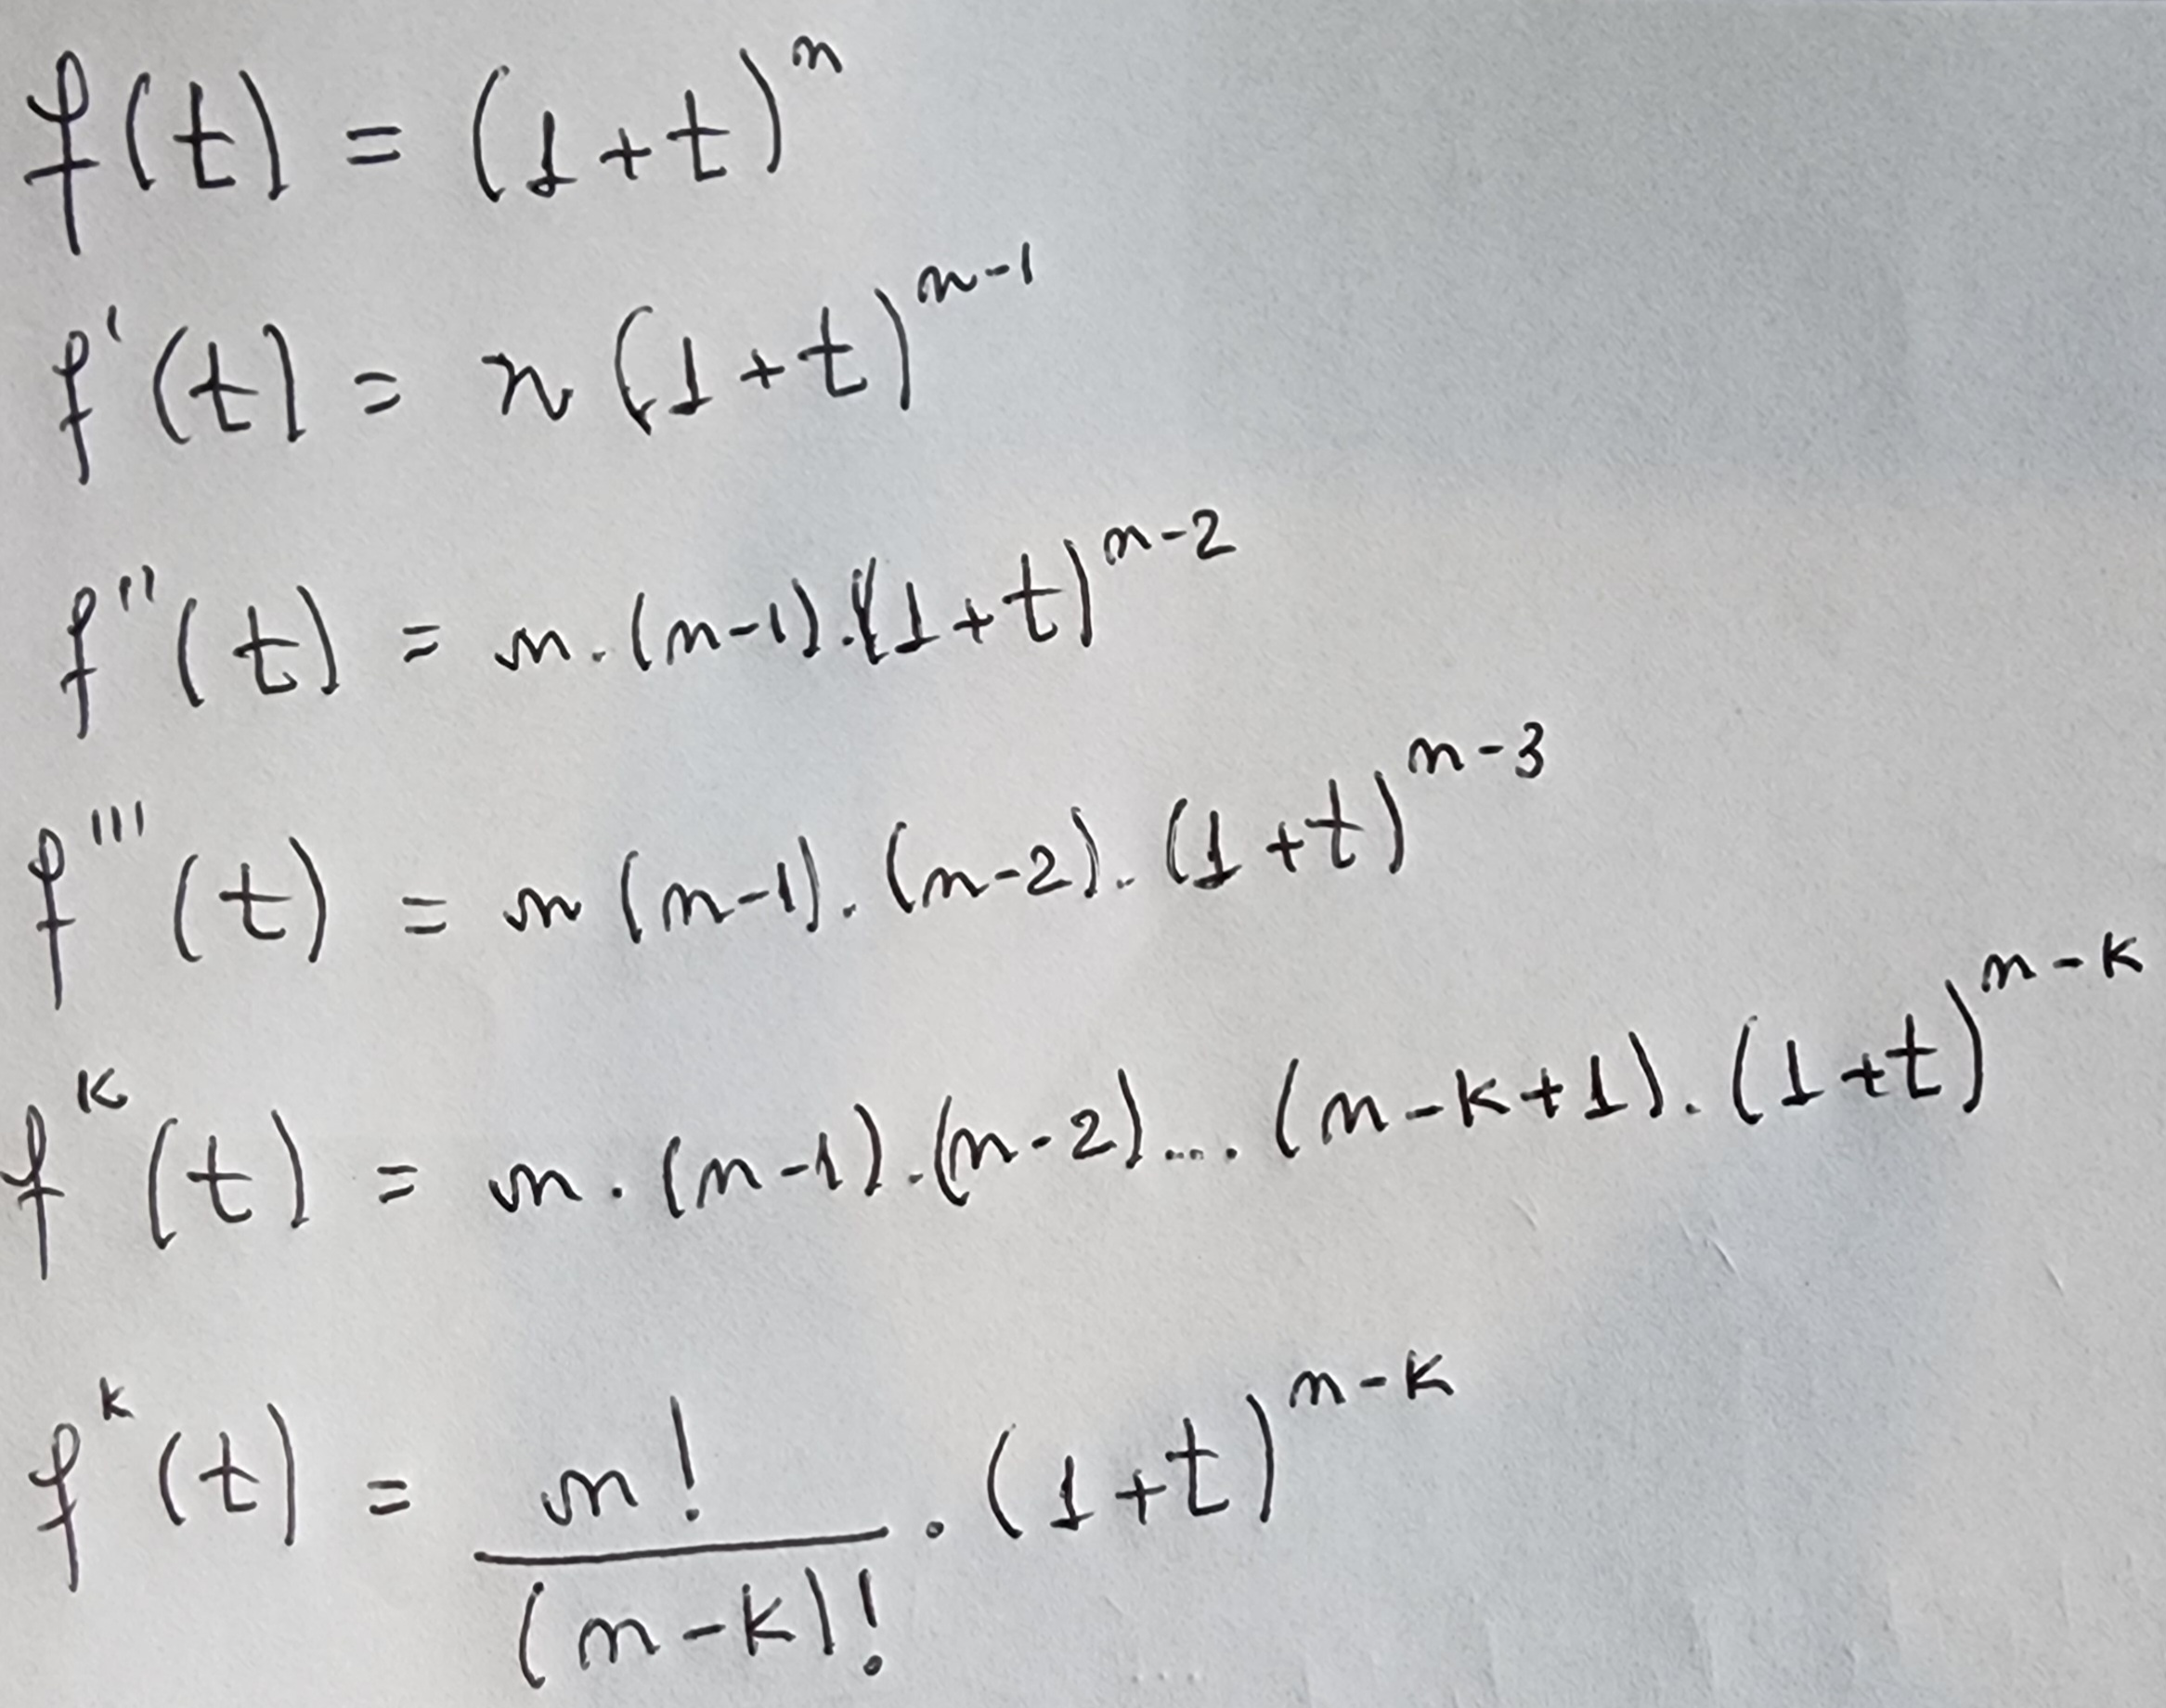
\includegraphics[width=1.0\textwidth]{imagens/exercicio2_parte1}
    \caption{Calculando as derivadas de $f(t)$ como resultado $f^{(k)}(t) = \frac{n!}{(n-k)!} \cdot (1 + t)^{n-k}$}
    \label{fig:exe2_parte1}
\end{figure}

\subsubsection{Descobrir quanto vale $f^{(k)}(0)$ de forma genérica.}
\begin{figure}[H]
    \centering
    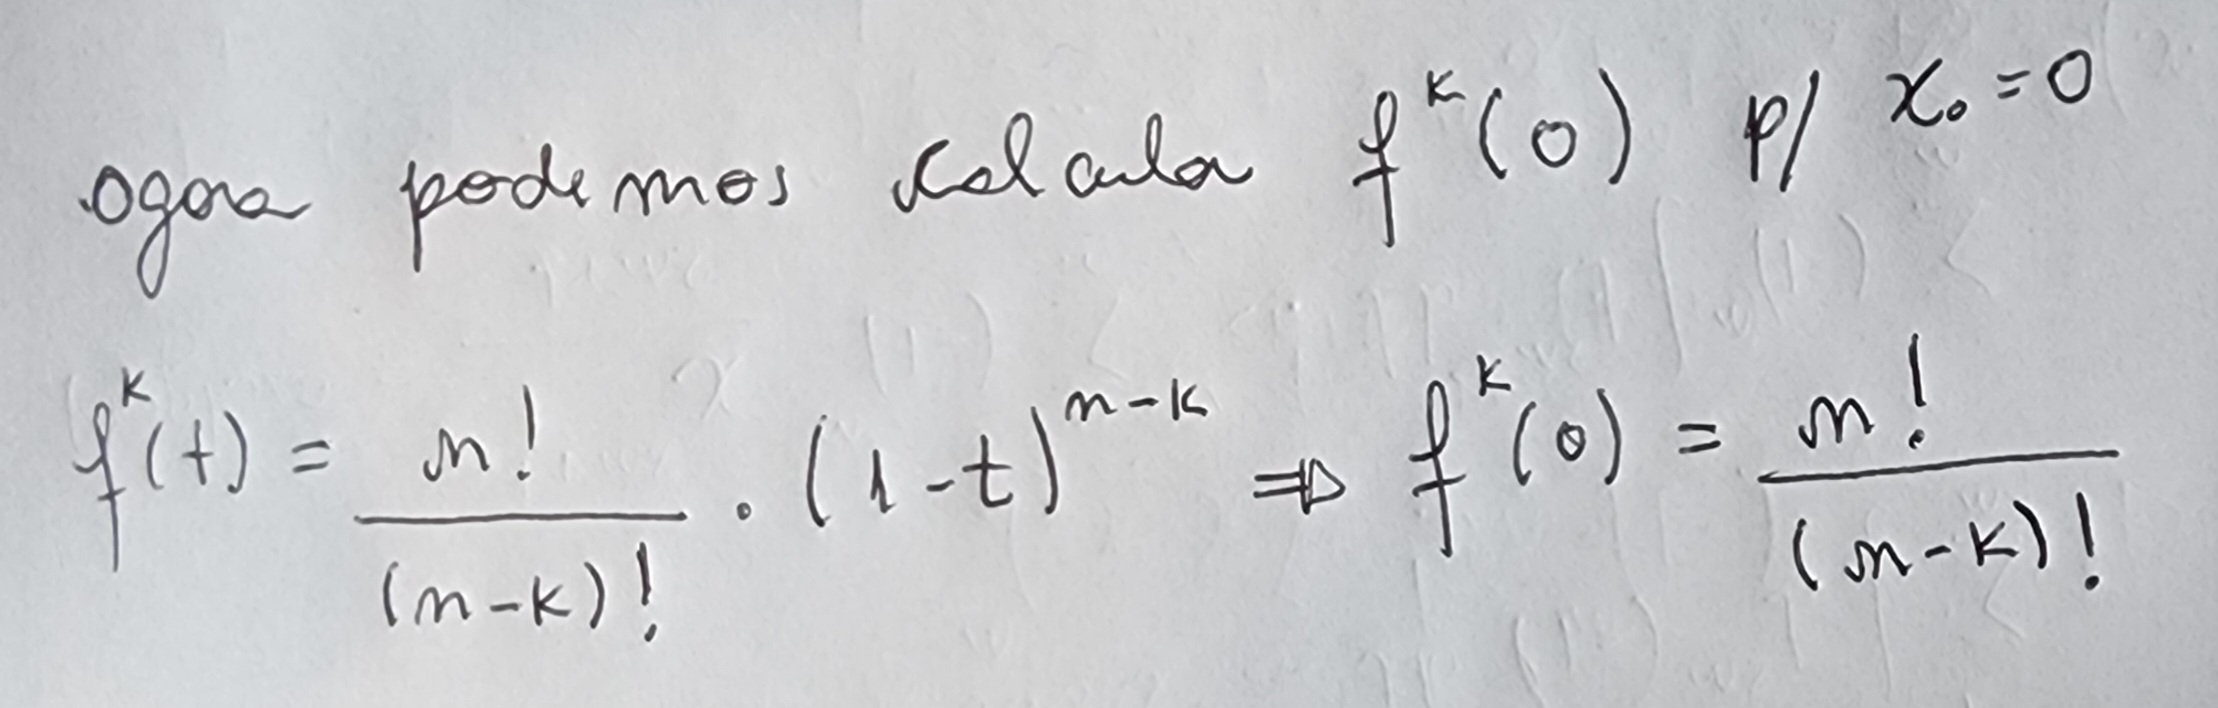
\includegraphics[width=1.0\textwidth]{imagens/exercicio2_parte2}
    \caption{Calculando $f^{(k)}(t)$ para $t = x_0 = 0$}
    \label{fig:exe2_parte2}
\end{figure}

\subsubsection{Expandir para a Série de taylor para forma genérica}
\begin{figure}[H]
    \centering
    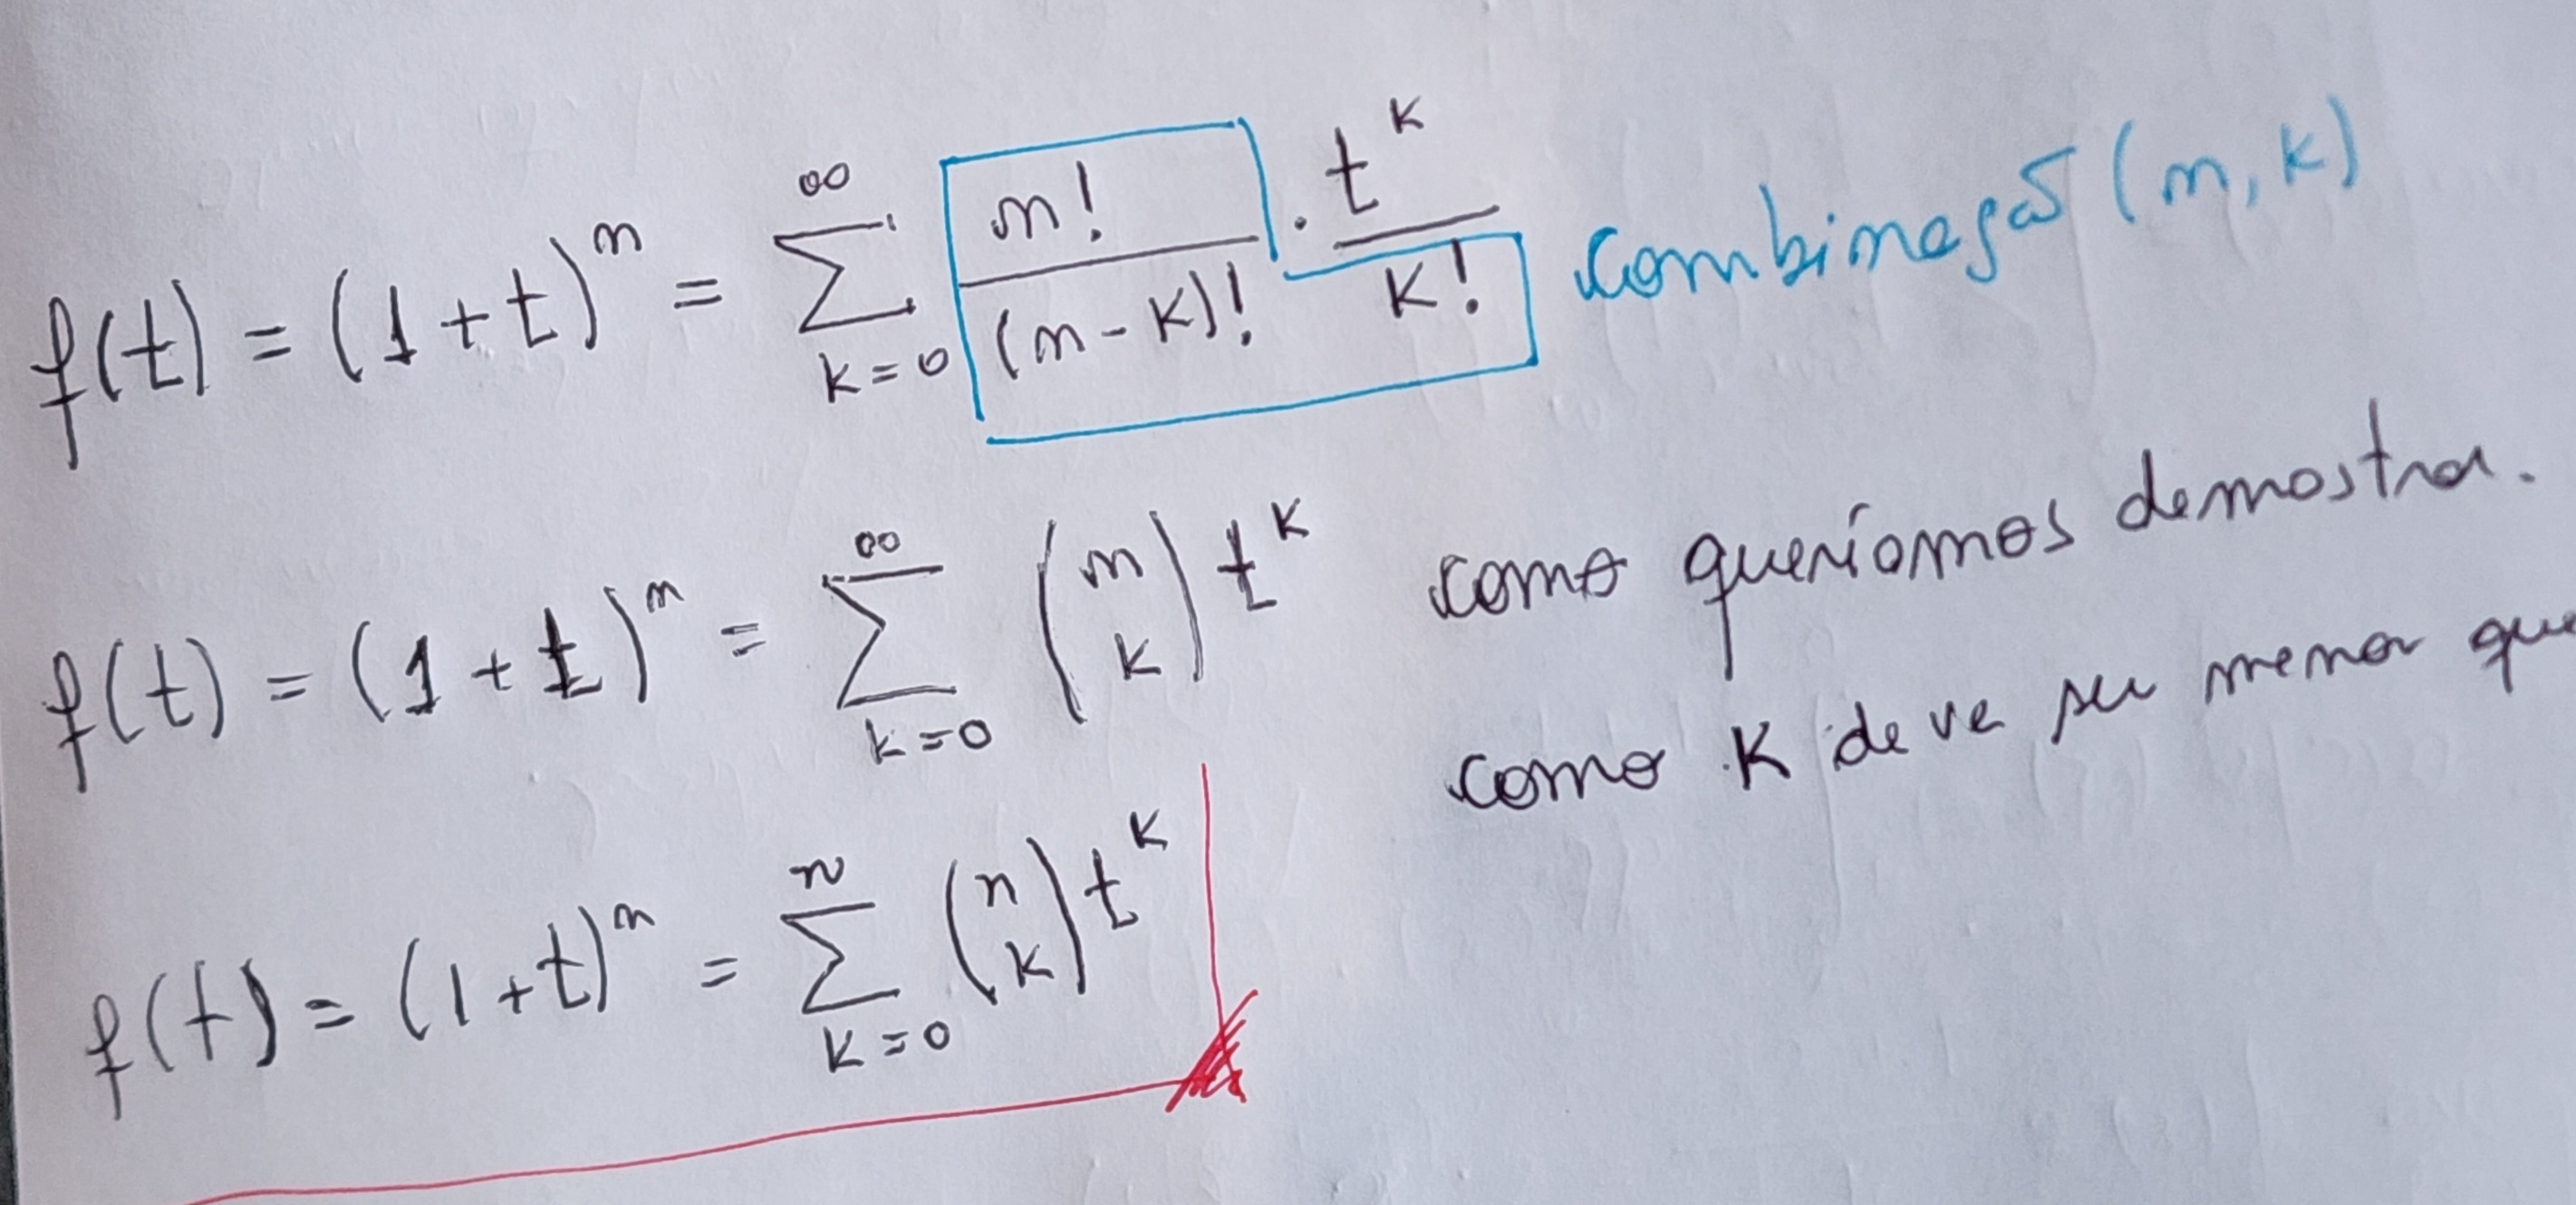
\includegraphics[width=1.0\textwidth]{imagens/exercicio2_parte3}
    \caption{Calculando $f(t)$ em para $t = x_0 = 0$ usando a Série de Taylor comprovando o enunciado.}
    \label{fig:exe2_parte3}
\end{figure}
Como k não pode ser maior que n, a última linha mostra que limitamos k entre 0 e n e não mais entre 0 e $\infty$

\subsubsection{Gerar tabela para comparação}

    \begin{table}[H]
    \centering
    \caption{Testes do Exercicio 2 com n = 10.}
    \label{tab:exercicio_2_resultados}
    \begin{tabular}{|c|c|c|c|}
    \toprule
    \textbf{$x$} & \textbf{$f(x,10)$} & \textbf{$P_k(x,10)$} & \textbf{Diferenca} \\
    \midrule   
    -1.0000e+01 & 3.4868e+09 & 3.4868e+09 & 0.0000000e+00 \\
                            -9.0000e+00 & 1.0737e+09 & 1.0737e+09 & 0.0000000e+00 \\
                            -8.0000e+00 & 2.8248e+08 & 2.8248e+08 & 0.0000000e+00 \\
                            -7.0000e+00 & 6.0466e+07 & 6.0466e+07 & 0.0000000e+00 \\
                            -6.0000e+00 & 9.7656e+06 & 9.7656e+06 & 0.0000000e+00 \\
                            -5.0000e+00 & 1.0486e+06 & 1.0486e+06 & 0.0000000e+00 \\
                            -4.0000e+00 & 5.9049e+04 & 5.9049e+04 & 0.0000000e+00 \\
                            -3.0000e+00 & 1.0240e+03 & 1.0240e+03 & 0.0000000e+00 \\
                            -2.0000e+00 & 1.0000e+00 & 1.0000e+00 & 0.0000000e+00 \\
                            -1.0000e+00 & 0.0000e+00 & 0.0000e+00 & 0.0000000e+00 \\
                            0.0000e+00 & 1.0000e+00 & 1.0000e+00 & 0.0000000e+00 \\
                            1.0000e+00 & 1.0240e+03 & 1.0240e+03 & 0.0000000e+00 \\
                            2.0000e+00 & 5.9049e+04 & 5.9049e+04 & 0.0000000e+00 \\
                            3.0000e+00 & 1.0486e+06 & 1.0486e+06 & 0.0000000e+00 \\
                            4.0000e+00 & 9.7656e+06 & 9.7656e+06 & 0.0000000e+00 \\
                            5.0000e+00 & 6.0466e+07 & 6.0466e+07 & 0.0000000e+00 \\
                            6.0000e+00 & 2.8248e+08 & 2.8248e+08 & 0.0000000e+00 \\
                            7.0000e+00 & 1.0737e+09 & 1.0737e+09 & 0.0000000e+00 \\
                            8.0000e+00 & 3.4868e+09 & 3.4868e+09 & 0.0000000e+00 \\
                            9.0000e+00 & 1.0000e+10 & 1.0000e+10 & 0.0000000e+00 \\
                            1.0000e+01 & 2.5937e+10 & 2.5937e+10 & 0.0000000e+00 \\
                            
    \bottomrule
    \end{tabular}
    \end{table}    
    
\newpage

\subsubsection{Apresentar o código Python}
\lstinputlisting[style=python]{scripts/exercicio2.py}
Código para testar a solução do exercício 2.


